\documentclass[11pt,a4paper]{scrartcl}
\usepackage[top=2cm,bottom=3cm,left=2cm,right=2cm]{geometry}
\usepackage{fontspec}
\usepackage{polyglossia}
    \setdefaultlanguage{english}
\usepackage{lmodern}
\usepackage{fixcmex}
\usepackage{enumitem}
\usepackage{mathtools}
\usepackage{amsmath}
\usepackage{amssymb}
\usepackage{amsfonts}
% \usepackage{bbold}
\usepackage{dsfont}
\usepackage{stmaryrd}
\usepackage{physics}
\usepackage{siunitx}
    \sisetup{%
        range-units=single,
        range-phrase={\text{~to~}},
        list-final-separator={\text{~and~}},
        separate-uncertainty=true,
        math-micro=\text{\textmu},
        text-micro=\textmu,
        math-ohm=\Omega,
        text-ohm=\ensuremath{\Omega},
    }
\usepackage{textcomp}
\usepackage{gensymb}
\usepackage{wasysym}
\usepackage[version=4]{mhchem}
\usepackage{csvsimple}
\usepackage{array}
\usepackage{booktabs}
\usepackage{graphicx}
    \graphicspath{{./img/}}
\usepackage{float}
\usepackage{caption}
\usepackage{subcaption}
\usepackage[parfill]{parskip}
\usepackage{nth}
\usepackage{csquotes}

\usepackage{tikz}
    \usetikzlibrary{%
        calc,
        external,
        graphs,
        plotmarks
    }
    \tikzexternalize[prefix=extern/]
    \tikzexternaldisable
\usepackage{pgfplots}
\usepackage{pgfplotstable}
    \usepgfplotslibrary{%
        colorbrewer,
        groupplots,
    }
\pgfplotsset{%
    compat=1.16,
    table/search path={plotdata},
    label style={font=\small},
    tick label style={font=\footnotesize},
    colormap/Set1-5,
    colormap/Dark2,
    log origin=infty,
    every axis/.append style={%
        tick style={semithick},
        legend style={font=\small}
    },
}
\usepackage[outputdir=latex_build]{minted}
    \usemintedstyle{friendly}
\usepackage{todonotes}
    \let\todox\todo
    \renewcommand{\todo}[1]{\todox[inline]{#1}}
\usepackage[colorlinks=true,linkcolor=blue]{hyperref}
\usepackage{cleveref}

\usepackage[%
    backend=biber,
    natbib=true,
    sorting=nyt,
    url=false,
    doi=true,
    isbn=false,
    maxbibnames=3,
    maxcitenames=2,
    date=year,
    urldate=iso,
    seconds=true,
    style=numeric-comp,
    autocite=superscript,
]{biblatex}
\addbibresource{literature.bib}



\DeclareMathOperator{\Ex}{\ensuremath{\mathbb{E}}}
\DeclareMathOperator{\Var}{Var}

\DeclareSIUnit{\gauss}{G}
\DeclareSIUnit{\parsec}{pc}

\newcommand\numberthis{\addtocounter{equation}{1}\tag{\theequation}}
\newcommand{\CRPropa}{\texttt{CRPropa}}
\newcommand{\inrange}[4]{\SIrange[range-phrase=\ensuremath{\le{#1}\le}]{#2}{#3}{#4}}
\newcommand{\Lamor}{\ensuremath{r_{\mathrm{L}}}}
\newcommand{\Brms}{\ensuremath{B_{\mathrm{rms}}}}
\newcommand{\kmin}{\ensuremath{k_{\mathrm{min}}}}
\newcommand{\kmax}{\ensuremath{k_{\mathrm{max}}}}
\newcommand{\lmin}{\ensuremath{l_{\mathrm{min}}}}
\newcommand{\lmax}{\ensuremath{l_{\mathrm{max}}}}
\newcommand{\pitch}{\ensuremath{\theta_{\mathrm{pitch}}}}
\newcommand{\Pesc}{\ensuremath{P_{\mathrm{esc}}}}
\newcommand{\CR}{\mathrm{CR}}
\newcommand{\pt}{\ensuremath{\partial_t}}
\newcommand{\Div}{\ensuremath{\nabla\cdot}}
\newcommand{\MA}{\ensuremath{\mathcal{M}_{\mathrm{A}}}}
\newcommand{\Mc}{\ensuremath{\mathcal{M}_{cs}}}
\newcommand{\MAsq}{\ensuremath{\MA^2}}
\newcommand{\Mcsq}{\ensuremath{\Mc^2}}
\renewcommand{\vec}[1]{\ensuremath{\mathbf{#1}}}
\newcommand{\Fe}{\ce{^{56}Fe}}
\newcommand{\alphaflat}{\alpha_{\mathrm{flat}}}
\newcommand{\alphafermi}{\alpha_{\mathrm{Fermi}}}
\newcommand{\ie}{i.\,e.}
\newcommand{\eg}{e.\,g.}



\titlehead{Ruhr-Universität Bochum, SS 2019}
\subject{\vspace*{-\baselineskip}Fortgeschrittenen-Praktikum: Theorie (804)}
\title{Acceleration and Propagation of Cosmic Rays}
\subtitle{}
\author{Jeremiah Lübke, 108015230366}
\date{\today}
\publishers{Advisor: Dr.~Björn Eichmann}



\begin{document}

\maketitle

\vspace{-1.7\baselineskip}
\noindent\rule{\textwidth}{1.2pt}
% \newpage

\setcounter{tocdepth}{2}
\tableofcontents

\newpage

\section{Introduction}
Cosmic Rays are protons and atomic nuclei with energies in the range
\SIrange{1e9}{1e21}{\electronvolt}, which move through space with nearly the
speed of light. Their spectrum (see \cref{fig:cr-whole-spectrum}) closely
resembles a power-law $j(E)\propto E^{-\alpha}$, on the basis of which one
can discuss some of their features:
\begin{itemize}
    \item At $E\sim\SI{1e15}{\electronvolt}$ (the \emph{knee}) the exponent
        steepens from $\alpha={2.5}\ldots{2.7}$ to $\alpha\approx3.1$;
        particles below this point can be detected directly, their flux is
        significantly anisotropic and their chemical composition is well
        understood.
    \item At $E\sim\SI{1e17}{\electronvolt}$ (the \emph{\nth{2} knee}) the
        exponent steepens again to $\alpha\approx3.3$.
    \item Particles with energies $\ge\SI{1e16}{\electronvolt}$ can not be
        observed directly, instead when colliding with molecules in the upper
        atmosphere a cascade of secondary particles is triggered
        (\emph{extensive air showers}; one primary cosmic rays produces
        $\ge\num{1e6}$ secondary particles). This makes it difficult to
        estimate their chemical composition, however current data strongly
        suggests that heavier nuclei are included. Their sources are as of
        today mostly uncertain.
    \item $E\sim\SI{1e18.5}{\electronvolt}$ is revered to as the \emph{ankle};
        there the exponent flattens to $\alpha\approx2.5$. With arrival rates
        of 1 particle km$^{-1}$ century$^{-1}$ at
        $E\sim\SI{1e19.5}{\electronvolt}$, the investigation of this range of
        the spectrum poses major challenges; the respective error bars in
        \cref{fig:cr-whole-spectrum-high} are of statistical nature.
    \item While for \inrange{E}{1e16}{1e19}{\electronvolt} the arrival
        directions are isotropic with a high confidence, recently
        significant anisotropies for $E\ge\SI{8e18}{\electronvolt}$ have been
        observed.
\end{itemize}

\begin{figure}[ht]
    \centering
    \begin{subfigure}[b]{.45\textwidth}
        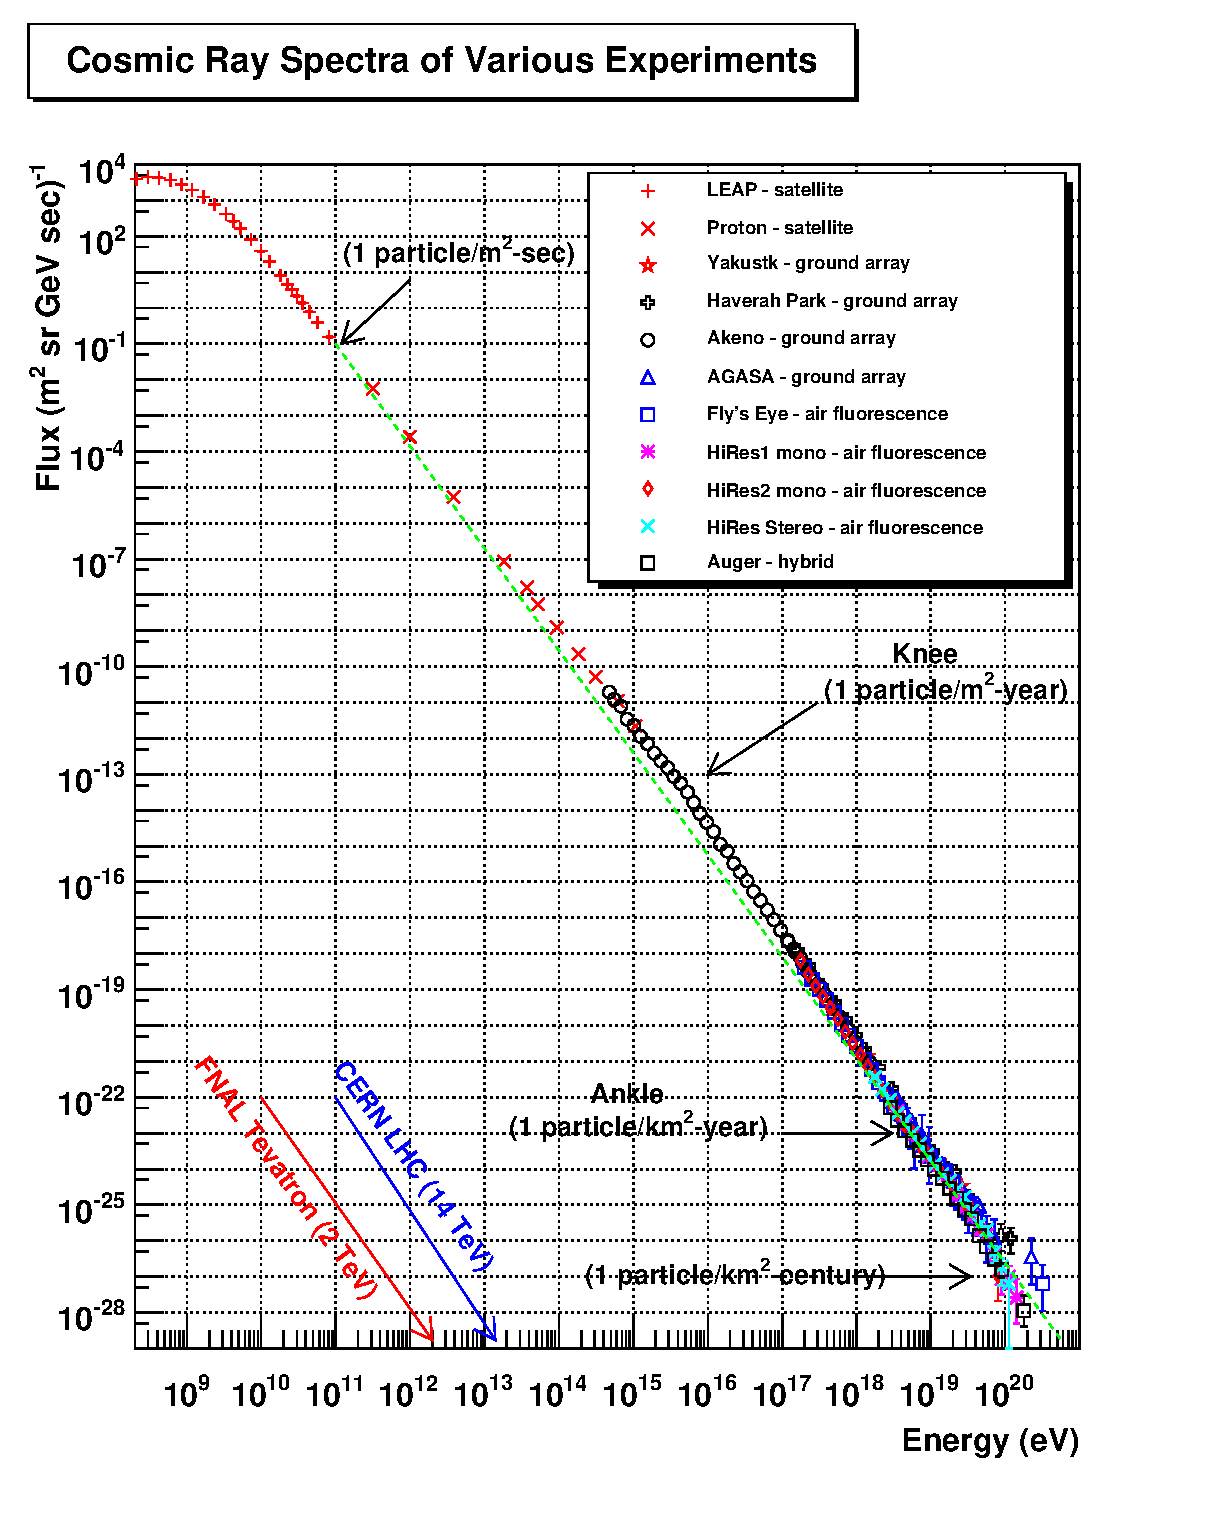
\includegraphics[width=\textwidth]{spectrum1}
        \caption{complete spectrum}
        \label{fig:cr-whole-spectrum-all}
    \end{subfigure}
    ~
    \begin{subfigure}[b]{.45\textwidth}
        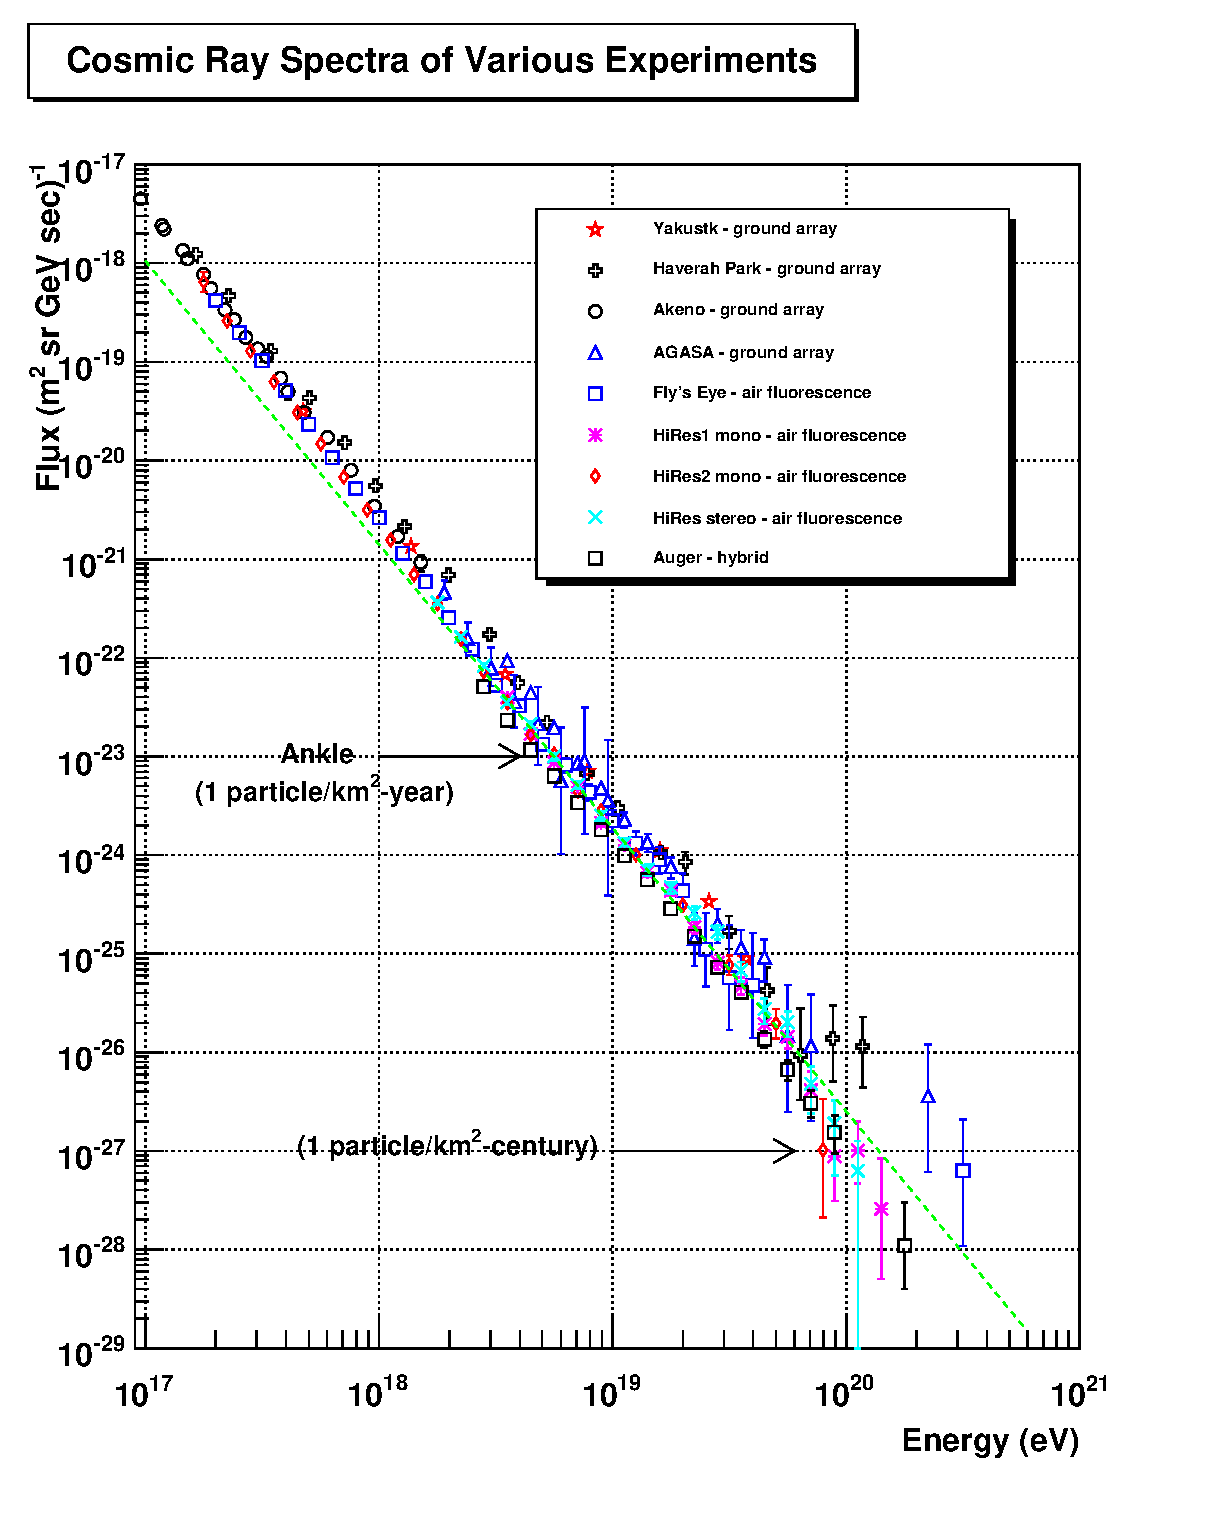
\includegraphics[width=\textwidth]{spectrum2}
        \caption{ultra-high energy regime}
        \label{fig:cr-whole-spectrum-high}
    \end{subfigure}
    \caption{Cosmic ray spectra of various experiments.
        Source\autocite{spectrum}}
    \label{fig:cr-whole-spectrum}
\end{figure}

This experiment is concerned with investigating the propagation of UHECR
(\emph{Ultra High Energy Cosmic Ray}) particles with energies above
\SI{1e18}{\electronvolt} using the Monte-Carlo code \CRPropa.


\section{Physical Fundamentals}
\subsection{Origin of UHECRs}
Which phenomenon is in principle able to accelerate particles to such large energies
(for reference: a particle with $E=\SI{3e20}{\electronvolt}$ has 23 million
times the LHC's collision energy of
$E_{\mathrm{LHC}}=\SI{13e12}{\electronvolt}$, but is still 40 million times
lower than the Planck energy $E_{\mathrm{P}}=\SI{1.2209e28}{\electronvolt}$)?

The isotropic distribution of arrival directions for particles with energies
$\ge\SI{1e16}{\electronvolt}$ suggests extra-galactic origins. This claim can
be supported by estimating the Lamor-radius of UHECRs (in the
ultra-relativistic limit with $E\approx pc$) in the interstellar magnetic
field: \begin{equation}
    \Lamor=\frac{p}{ZeB}=\frac{E}{ZeBc}
\end{equation}
With a representative average galactic magnetic field strength of
$\SI{10}{\micro\gauss}$, one finds the values listed in \cref{tab:Lamor}.
Looking at these values, one finds that they are comparable to the estimated
half-thickness of the milky way's stellar disk of \SI{300}{\parsec} and its
radius of \SI{30}{\kilo\parsec}. One can argue, that as as soon as a particle's
Lamor-radius exceeds the half-thickness of it's source galaxy, it is able to
escape the galaxy's magnetic field.

\begin{table}[ht]
    \centering
    \sisetup{table-parse-only}
    \begin{tabular}{SSS}
        \toprule
        {$E/\si{\eV}$} & {$\Lamor/\si{\parsec}$ of a Proton} &
        {$\Lamor/\si{\parsec}$ of a \ce{^{56}Fe} nucleus} \\
        \midrule
        1e15 & .108 & 4.16e-3 \\
        1e17 & 10.8 & .416 \\
        1e19 & 1.08e3 & 41.6 \\
        1e21 & 108e3 & 4.16e3 \\
        \bottomrule
    \end{tabular}
    \caption{Lamor-radii for UHECR protons and iron nuclei with
        $B=\SI{10}{\micro\gauss}$}
    \label{tab:Lamor}
\end{table}

One class of possible extra-galactic particle accelerators are Active Galactic
Nuclei (AGN), which refer to galactic centers which outshine their host
galaxies and constitute the most luminous objects in the Universe. AGNs are
believed to be powered by mass-accreting super-massive black holes. Some of the
such arising accretion disks produce relativistic jets, \ie~highly collimated
beams of ionised particles accelerated close to the speed of light.
Additionally in such jet structures internal and external shocks might further
accelerate those particles. However the data available to date does not
sufficiently correlate the detected CRs with this kind of source.

Other possible sources include neutron stars, relativistic supernovae,
gamma-ray bursts or (going beyond the standard model) decay products of
super-massive topological defects in the underlying quantum field.


\subsection{Acceleration of Particles at Shocks}
Now, which processes are able to accelerate cosmic rays in such a way, that the
observed power spectrum is produced?
Promising candidates are astrophysical shocks, both locally (such as in solar
flares or relativistic jets) and on large scales (such as supernovae or
AGN), which was first described by Fermi (focusing on large-scale
phenomena)\autocite{Fermi1949}.

Considering some test particle in the vicinity of a shock, which is assumed to
experience an energy gain proportional to its energy during each encounter with
the shock $\Delta{E}=\zeta{E}$ and an initial energy $E_0$, one finds:
\begin{align*}
    E_1&=E_0+\Delta{E_0}=E_0(1+\zeta)\qc&\text{after the \nth{1} encounter} \\
    E_2&=E_1+\Delta{E_1}=E_0(1+\zeta)+\zeta{E_0}(1+\zeta)=E_0(1+\zeta)^2
    \qc&\text{after the \nth{2} encounter} \\
    &\vdots& \\
    E_n&=E_0(1+\zeta)^n\qc&\text{after the $n^{\text{th}}$ encounter}
    \numberthis\label{eq:En}
\end{align*}
It follows from \cref{eq:En}, that
\begin{equation}
    n={\log\left(\frac{E}{E_0}\right)}/{\log(1+\zeta)}
    \label{eq:num-enc}
\end{equation}
encounters are required to reach some energy $E$.

In a similar manner one can show, that the probability to remain in the
vicinity of the accelerating shock is $(1-\Pesc)^n$, where \Pesc~denotes the
escape probability per encounter.
Then the number of particles accelerated to energies greater than $E$ is
proportional to the sum of probabilities to remain, starting at the minimal
energy after $n$ encounters and taking into account all higher orders. This
eventually leads to a power law as shown in \cref{sec:app1}:
\begin{equation}
    N(>E)\propto\sum_{m=n}^{\infty}(1+\Pesc)^m
    \propto\frac{1}{\Pesc}\left(\frac{E}{E_0}\right)^{-\alpha},
    \label{eq:N-power}
\end{equation}
where the spectral index is approximately given by (for $\Pesc,\zeta\ll1$):
\begin{equation}
    \alpha\approx\frac{\Pesc}{\zeta}.
    \label{eq:alpha}
\end{equation}

Writing \cref{eq:N-power} as a differential energy spectrum yields:
\begin{equation}
    \boxed{%
        \dv{N(>E)}{E}\propto\left(\frac{E}{E_0}\right)^{-\alpha-1}
    }
    \label{eq:N-diff}
\end{equation}

Now, in order to determine the energy gain factor $\zeta$, two mechanisms of
acceleration are taken under closer consideration.


\subsubsection{\nth{2} order Fermi acceleration}
At first encounters of an ultra-relativistic test particle with
a moving cloud of plasma is discussed, where \emph{encounter} means entering
and exiting the cloud (see \cref{fig:fermi2}).

\begin{figure}[ht]
    \centering
    \includegraphics[width=.5\textwidth]{fermi2}
    \caption{Acceleration by a moving plasma cloud. Source\autocite{Gaisser}}
    \label{fig:fermi2}
\end{figure}

The particle with energy $E_1$ enters the cloud and diffuses by collisionless
scattering (without energy loss) on the irregularities in the magnetic field,
in such a way, that its \emph{average} motion coincides with that of the cloud.
In the following, primed quantities denote the rest-frame of the cloud, while
un-primed quantities denote the laboratory frame and the indices
\emph{1}/\emph{2} denote the state before/after the encounter.
Therewith the particle has in the rest-frame of the cloud the total energy
\begin{equation}
    E_1'=\gamma E_1(1-\beta\cos\theta_1)
    \label{eq:fermi2-e1p}
\end{equation}
with the Lorentz factor $\gamma$, the cloud's velocity $\beta=V/c$ and the
angle between the particle's and the cloud's velocity at entry $\theta_1$.
At the point of exiting, the particle's energy is unchanged in the cloud's
rest-frame ($E_1'=E_2'$), since only elastic scattering took place.
Transforming back into the laboratory frame then yields as the particle's
energy after the encounter
\begin{equation}
    E_2=\gamma E_2'(1+\beta\cos\theta_2')
    \label{eq:fermi2-e2}
\end{equation}
where $\theta_2'$ is the angle between the particle's and the cloud's velocity
at exit.

Now with the difference of \cref{eq:fermi2-e1p,eq:fermi2-e2} the energy change
can be computed:
\begin{align*}
    \frac{\Delta{E}}{E_1}
    &=\frac{\gamma{E_2'}(1+\beta\cos\theta_2')-\frac{E_1'}{\gamma(1-\beta\cos\theta_1)}}{\frac{E_1'}{\gamma(1-\beta\cos\theta_1)}}
    =\gamma(1-\beta\cos\theta_1)\gamma(1+\beta\cos\theta_2')-1\\
    &=\frac{1-\beta\cos\theta_1+\beta\cos_2'-\beta^2\cos\theta_1\cos\theta_2'}{1-\beta^2}-1.
    \numberthis\label{eq:dE}
\end{align*}

In order to find the average fractional energy gain per encounter,
$\cos\theta_1$ and $\cos\theta_2'$ need to be averaged:
\begin{align*}
    \langle\cos\theta_2'\rangle
    &=\frac{\int_{\text{all directions}}\dd{n}\cos\theta_2'}{\int_{\text{all
    directions}}\dd{n}}
    =\frac{\int_{-1}^{+1}\dd{\cos\theta_2'}\dv{n}{\cos\theta_2'}\cos\theta_2'}{\int_{-1}^{+1}\dd{\cos\theta_2'}\dv{n}{\cos\theta_2'}}
    =0,\numberthis
\end{align*}
since particles can leave the cloud isotropically, \ie~the probability for the
direction of exit is constant
\begin{equation}
    \dv{n}{\cos\theta_2'}=\mathrm{const.}\qc-1\le\cos\theta_2'\le1.
\end{equation}
Next, the probability for a collision of a cloud and a particle is proportional
to their relative velocity (with $v_{\mathrm{particle}}\approx c$)
\begin{equation}
    \dv{n}{\cos\theta_1}=\frac{c-V\cos\theta_1}{2c}\qc-1\le\cos\theta_1\le1,
\end{equation}
which gives
\begin{align*}
    \langle\cos\theta_1\rangle
    &=\frac{\int_{-1}^{+1}\dd{\cos\theta_1}\frac{c-V\cos\theta_1}{2c}\cos\theta_1}{\int_{-1}^{+1}\dd{\cos\theta_1}\frac{c-V\cos\theta_1}{2c}}
    =-\frac{V}{2c}\left[\frac{x^3}{3}\right]_{-1}^{+1}
    =-\frac{V}{3c}=-\frac{\beta}{3}.\numberthis
\end{align*}
Finally, one receives for the energy gain factor
\begin{equation}
    \zeta=\frac{\langle\Delta{E}\rangle}{E_1}
    =\frac{1+\frac{1}{3}\beta^2}{1-\beta}-1=\frac{\frac{4}{3}\beta^2}{1-\beta^2}
    \approx\frac{4}{3}\beta^2
    \label{eq:gain2}
\end{equation}
with the last approximation being valid for non-relativistic clouds,
\ie~$\beta\ll1$.

On average, particles gain energy according to \cref{eq:gain2}, however in
single encounters a particle might gain or lose energy depending on the entry
and exit angles.


\subsubsection{\nth{1} order Fermi acceleration}
The second situation deals with acceleration by a plane (infinitely spread out)
shock front moving with velocity $-\vec{u_1}$ (see \cref{fig:fermi1}).
The area in front of the shock is referred to as \emph{upstream} and the area
behind as \emph{downstream} region. The (shocked) downstream plasma moves away
from the shock front with velocity $\vec{u_2}$, where $u_2<u_1$, thus its
velocity in the lab frame is $\vec{V}=-\vec{u_1}+\vec{u_2}$.
Similar as above, \emph{encounter} means moving in and out of the shocked
region.

\begin{figure}[ht]
    \centering
    \includegraphics[width=.5\textwidth]{fermi1}
    \caption{Acceleration at a plane shock front. Source\autocite{Gaisser}}
    \label{fig:fermi1}
\end{figure}

\Cref{eq:dE} can still be applied here, with $\beta=V/c$ referring to the
downstream velocity. However when averaging the angular distributions, the
isotropy of entering and exiting directions only applies to the area behind or
in front of the shock respectively, \ie~the angles $\theta_2'$ and $\theta_1$
only take values in $[0,\pi/2]$ and $[-\pi/2,0]$ respectively and
the probabilities need to be projected onto the shock front and normalized
properly:
\begin{gather}
    \dv{n}{\cos\theta_2'}=2\cos\theta_2'\qc0\le\cos\theta_2'\le1 \\
    \dv{n}{\cos\theta_1}=2\cos\theta_1\qc-1\le\cos\theta_1\le0 \\
    \implies\langle\cos\theta_2'\rangle=-\langle\cos\theta_1\rangle=\frac{2}{3},
\end{gather}
which eventually yields for the energy gain factor
\begin{equation}
    \zeta=\frac{\langle\Delta{E}\rangle}{E_1}
    =\frac{1+\frac{4}{3}\beta+\frac{4}{9}\beta^2}{1-\beta^2}-1
    \approx\frac{4}{3}\beta=\frac{4}{3}\frac{u_1-u_2}{c},
    \label{eq:gain1}
\end{equation}
with the last approximation being valid for non-relativistic shocks,
\ie~$\beta\ll1$.

Due to the angular constraints, encounters with a plane shock front always
result in an energy gain.


\subsubsection{Acceleration at plane shock fronts}
The cosmic ray flux, which is to be accelerated by a shock front, first passes
from the upstream to the downstream region. This flux is found by projecting
some initially isotropic flux
$F_{\CR}^{\mathrm{iso}}=c\rho_{\CR}/4\pi$ onto the plane shock
front:
\begin{equation}
    F_{\CR}^{u\to{d}}
    =\int\limits_0^1\int\limits_0^{2\pi}\dd{\cos\theta}\dd{\phi}
    F_{\CR}^{\mathrm{iso}}\cos\theta
    =\int\limits_0^1\int\limits_0^{2\pi}\dd{\cos\theta}\dd{\phi}
    \frac{c\rho_{\CR}\cos\theta}{4\pi}
    =\frac{c\rho_{\CR}}{4}.
\end{equation}
The CR flux, which escapes from the shock front and is not being further
accelerated is given by the flux, which is on average transported away from the
shock front by the downstream plasma with speed $u_2$,
\ie~$F_\CR^{\mathrm{esc}}=\rho_{\CR}u_2$. The probability to
escape the region of acceleration is equal to the ratio of the fluxes, which
escape and which enter that region:
\begin{equation}
    \Pesc=\frac{F_{\CR}^{\mathrm{esc}}}{F_{\CR}^{u\to{d}}}
    =\frac{\rho_\CR u_2}{c\rho_\CR/4}=\frac{4u_2}{c}
    \label{eq:Pesc}
\end{equation}

Having estimated the energy gain factor \cref{eq:gain1} and the escape
probability \cref{eq:Pesc}, the spectral index \cref{eq:alpha} can finally be
obtained:
\begin{equation}
    \alpha=\frac{\Pesc}{\zeta}=\frac{4u_2/c}{4(u_1-u_2)/3c}=\frac{3}{u_1/u_2-1},
    \label{eq:alpha-plane-shock}
\end{equation}
where the ratio $u_1/u_2$ denotes the \emph{compression ratio} $r$ of the
shock. For a perpendicular MHD shock in the limit of large upstream flow
energy, one has (as shown in \cref{sec:app2}):
\begin{equation}
    r=\frac{\gamma+1}{\gamma-1}.
\end{equation}
Assuming mono-atomic gas with adiabatic index $\gamma=5/3$ gives $r=4$, \ie~for
the aforementioned assumptions the maximum jump of the plasma quantities at the
discontinuity of the shock is by a factor of four.

Therewith the spectral index becomes $\alpha=1$ and yields for the
differential energy spectrum \cref{eq:N-diff}:
\begin{equation}
    \boxed{\dd{N}\propto E^{-2}\dd{E}}
    \label{eq:N-power-2}
\end{equation}


\subsection{GZK Cutoff}
The here investigated UHECR protons have such large Lorentz factors, that the
photons of the Cosmic Microwave Background (CMB) get blue-shifted into the
$\gamma$-regime in the proton's rest frame.
With the proton being bombarded by high-energy $\gamma$-photons, pions are
created:
\begin{align*}
    \ce{p + $\gamma$ &-> n + $\pi^+$ -> n + $\nu^+ + \nu_{\mu}$} \\
    \ce{p + $\gamma$ &-> p + $\pi^0$ -> p + $\gamma + \gamma$}
\end{align*}
Integrating over the black-body spectrum of the CMB and over all angles, one
finds the threshold for \textbf{Photo-Pion Production} to be
$E\approx\SI{5e19}{\electronvolt}$. Further the mean free path for a single
scattering with a CMB photon can be estimated to
$\lambda\approx\SI{1e23}{\metre}\approx\SI{3}{\mega\parsec}$. The energy of the
so created pion is $\gamma m_{\pi} c^2$ and thus the fractional energy loss of
the proton is $\Delta{E}/E\approx m_{\pi}/m_p\approx 1/10$. Therefore, the
total mean free path for the proton to loose all its energy is about
\SI{30}{\mega\parsec}, which means there must be a cutoff in the energy
spectrum at \SI{5e19}{\electronvolt} if the cosmic rays originate from further
away (as first discussed by Greisen, Kuz'min and Zatsepin). However no such
cutoff is apparent in the measured spectrum, which means that either the cosmic
rays sources are located closer than \SI{30}{\mega\parsec} or the cosmic rays
are constituted of heavier nuclei such as iron instead of protons, which would imply
a smaller Lorentz factor for the same particle energy and thus the cutoff being
located at even higher energies.

Another process is $e^-$-$e^+$ \textbf{Photo-Pair Production}, where a
$\gamma$-photon with at least twice the rest energy of an electron is converted
into an electron and a positron. This only happens in the vicinity of a
heavier particle (such as a proton or heavier nucleus) in order to account for
conservation of momentum. A similar calculation as above can be carried out for
this process to yield a threshold for the proton energy of about
\SI{1e18}{\electronvolt}. While the cross-section here is 40 times larger
compared to photo-pion production, the fractional energy loss of the proton is
only $\Delta{E}/E\approx10^{-3}$, causing a 25 times longer
loss-scale.

In the case of the UHECRs being nuclei, \textbf{Photo-Disintegration} needs
also to
be considered: when the $\gamma$-photons in the rest frame of the nucleus reach
energies comparably to the binding energy per nucleon (which is of order
\SI{10}{\mega\electronvolt}), the absorption of such a photon leads to the
excitation of one or two nucleons and their subsequent ejection from the
nucleus. The smaller nucleus afterwards continues its disintegration via
further photo-disintegration and radioactive decay. From the Lorentz factor
necessary for this process, one finds for the threshold energy
$E\ge{A\times10^{18}}\si{\electronvolt}$, leading to a expected cutoff at about
\SIrange{1e19}{1e20}{\electronvolt}. The associated loss-scale is expected to
be smaller than with photo-pion production.

All of the above processes can also occur in interaction with Cosmic Infrared
Background (IRB), which is mostly due to galaxy formation and starlight absorbed
and re-emitted by interstellar dust. The hereafter performed simulations
use the model by Gilmore\autocite{Gilmore2012}.


\subsection{Turbulent Magnetic Fields}
\label{sec:intro-turbulence}
At first -- from a naive perspective -- the observed isotropy is unexpected, as
one would expect particles with such high energies to not be significantly
affected by magnetic fields and point directly back to their sources. That this
is not the case, can be explained by resonant scattering of those particles
with turbulent magnetic fields.

How generation and maintenance of large-scale magnetic fields in the Universe
theoretically work, is still unsolved as of today. Additionally -- while the
large-scale structure of galactic magnetic fields can be understood by
measuring the polarization of synchrotron radiation and taking Faraday rotation
into account -- putting observational constrains on the field strength
of extra-galactic magnetic fields is rather difficult.

For simplicity in this experiment a uniform isotropic turbulent field is
assumed, which is characterized by the root mean squared strength
$\Brms=\sqrt{\langle{B^2(x)}\rangle}$ and the distribution of magnetic energy
$w$, which -- according to Kolmogorov theory -- follows a power-law in Fourier
space between the maximum and minimum wave-numbers \kmin~and \kmax, which
describes how much energy is contained in eddies with wave-number $k$:
\begin{equation}
    w(k)=\frac{\Brms^2}{8\pi}k^{-m}\frac{(m-1)\kmin^{m-1}}{1-(\kmax/\kmin)^{m-1}},
\end{equation}
where a Kolmogorov spectrum with spectral index $m=5/3$ is chosen.
In a turbulent system energy is injected at the maximum length scale
$\lmax=2\pi/\kmin$ and from there is transferred through wave interactions to
the minimum length scale $\lmin=2\pi/\kmax$, where it dissipates.
Additionally, one can compute the correlation length $l_c$, which is the
characteristic length scale on which the magnetic field varies, and can be
thought of as roughly the size of the largest eddy in the system. For uniform
isotropic turbulent flow, Kolmogorov turbulence and $\lmin\ll\lmax$ one has:
\begin{equation}
    l_c=\frac{8\pi^2}{\Brms^2}\int\limits_{0}^{\infty}\frac{\dd{k}}{k}w(k)
    =\frac{\lmax}{2}\frac{m-1}{m}\frac{1-(\lmin/\lmax)^m}{1-(\lmin/\lmax)^{m-1}}
    \approx\frac{\lmax}{5}.
\end{equation}

A useful quantity to classify the relation of the particle with the magnetic
field is the dimensionless rigidity $\rho=\Lamor/l_c$, where $\Lamor=E/Ze\Brms
c$ is the particle's Lamor-radius in the ultra-relativistic limit.

Now, the particle undergoes resonant scattering if $k\cos\pitch=1/\Lamor$:
\begin{itemize}
    \item upper limit:
        \[\kmin\le\frac{1}{\Lamor} \implies \rho\le\frac{5}{2\pi}\approx1\]
        $\rho\approx1$ divides the resonant from the quasi-ballistic regime; for
        $\rho\gg1$ the particle propagates quasi-rectilinear.
    \item lower limit:
        \[\kmax\ge\frac{1}{\Lamor} \implies
            \rho\ge\frac{5}{2\pi}\frac{\lmin}{\lmax}\approx\frac{\lmin}{\lmax}\]
        At $\rho\ll1$ particle propagation is also affected by magnetic field
        line random walks.
\end{itemize}
Therefore, the resonant scattering regime at which particle propagation is
diffusive is given by:
\begin{equation}
    \frac{\lmin}{\lmax}<\rho<1
    \label{eq:resontant-scattering}
\end{equation}


\subsection{Propagation of UHECRs}
\subsubsection{CRPropa3}
The propagation of cosmic rays can be obtained by solving either the
Fokker-Planck equation for a distribution of many particles
or the equation of motion according to the Lorentz force for a single particle.
Since for both cases no analytical solutions exist (due to the complicated
setting of the problem), one approaches this problem
numerically. With \CRPropa~a tool is provided for this task, which can compute
the propagation of cosmic rays -- including deflection by turbulent magnetic
fields, several energy loss processes through interaction with background
photon fields and nuclear decay -- over several orders of magnitude in energy
and length scales (hundreds of megaparsecs to kiloparsec).

Here the simplest case of solving the equation of motion of single particles is
considered, whose initial conditions are randomly drawn from a source probability
distribution. In order to obtain reliable results (\ie~with negligible
statistical fluctuations) this needs to be repeated for a large number of
particles.


\subsubsection{The Monte-Carlo method}
The basic idea behind the Monte-Carlo approach is to repeatedly perform an
experiment -- which is subject to random fluctuations (\eg~initial
conditions) -- a large amount of times and average the results. When
those \enquote{experiments} are cleverly designed, one is able to compute
difficult integrals (\emph{here:} the equations of motion of single
particles) easily without the need for a deep theoretical understanding of
the system under consideration.

Through the large amount of repetitions, the algorithm makes use of the
\emph{central limit theorem}, which states that the distribution of randomly
generated, independent experiments tends towards a normal distribution as the
number of experiments increases.
While normal distributions describe continuous random variables, Monte-Carlo
algorithms -- such as the here employed code \CRPropa~-- yield discrete results
describing how often an event occurs within a certain interval. Here those
events are particles, which are accumulated in energy bins.
Now, the probability of observing $k$ events in a given interval with $\lambda$
average events per interval is described by \emph{Poisson statistics}, whose
distribution is given by
\begin{equation}
    P(k)=e^{-\lambda}\frac{\lambda^k}{k!}.
    \label{eq:poisson}
\end{equation}

Note, that -- unlike a normal distribution -- the shape of a Poisson
distribution is not symmetric, however for large $\lambda$ a normal
distribution is approximated.

Further note, that for a Poisson-distributed random variable $X$ and real,
positive $\lambda$ the expected value and the variance are equal to $\lambda$:
\begin{equation}
    \Ex(X)=\sum_{k=0}^{\infty}k\,P(k)
    =\sum_{k=0}^{\infty}k\,e^{-\lambda}\frac{\lambda^k}{k!}
    =\lambda\,e^{-\lambda}
    \underbrace{\sum_{k=0}^{\infty}\frac{\lambda^{k-1}}{(k-1)!}}_{=e^{\lambda}}
    =\lambda
    \label{eq:poisson-exp}
\end{equation}
and
\begin{equation}
    \Var(X)=\Ex(X^2)-\Ex(X)^2=\lambda
    \label{eq:possion-var}
\end{equation}
with
\begin{align*}
    \Ex(X^2)&=\sum_{k=0}^{\infty}k^2\,e^{-\lambda}\frac{\lambda^k}{k!}
    =\lambda\,e^{-\lambda}\sum_{k=1}^{\infty}\frac{k\,\lambda^{k-1}}{(k-1)!}
    =\lambda\,e^{-\lambda}\sum_{l=0}^{\infty}\lambda^l\frac{l+1}{l!}
    \\
    &=\lambda\,e^{-\lambda}\left(
    \sum_{l'=0}^{\infty}\frac{\lambda^{l'}}{l'!}
    +\sum_{l=0}^{\infty}\frac{l\,\lambda^l}{l!}
    \right)
    =\lambda\,e^{-\lambda}\Bigg(
    e^{\lambda}+\lambda\underbrace{%
        \sum_{l=0}^{\infty}\frac{\lambda^{l-1}}{(l-1)!}}_{=e^\lambda}
    \Bigg)
    =\lambda+\lambda^2
\end{align*}

Now, considering a MC simulation with $n$ total events, out of which $k$ events
hit a certain energy bin, the expected average of this bin is $\lambda_n=k/n$.
Additionally, a single MC run yields a discrete result $Y_i$ and the average
and variance of $n$ such results is $\lambda_n=\frac{1}{n}\sum_{i=1}^{n}Y_i$
and $\Var(Y)=\sigma^2$, respectively.
The variance of the expected value $\lambda_n$ is then
\begin{equation}
    \Var(\lambda_n)=\Var\left(\frac{1}{n}\sum_{i=1}^{n}Y_i\right)
    =\frac{1}{n^2}\underbrace{\sum_{i=1}^{n}\Var(Y_i)}_{=n\sigma^2}
    =\frac{\sigma^2}{n}=\frac{\lambda_n}{k/\lambda_n}=\frac{\lambda_n^2}{k},
\end{equation}
where the Bienaymé relation
\begin{equation*}
    \Var\left(\sum_{i=1}^{n}Y_i\right)=\sum_{i=1}^{n}Y_i
\end{equation*}
and the property
\begin{equation*}
    \Var(aX)=a^2\Var(X)
\end{equation*}
have been employed and the variance $\sigma^2=\lambda_n$ was estimated
according to Poisson statistics.
Therewith the standard deviation for the average number of events per interval
becomes
\begin{equation}
    \Delta\lambda_n=\frac{\lambda_n}{\sqrt{k}}.
    \label{eq:mc-std}
\end{equation}

\emph{Note:} due to the random nature of MC simulations there is no
difference between one run with $n$ events and $n$ runs with one event each.


\subsubsection{Reweighting}
A common technique used in experiments and MC simulations is the reweighting of
an initial distribution.

In the case of \CRPropa, particles with energies from a given initial
distribution are propagated to some observer. During this process, the
particles suffer energy losses and only a small amount actually reaches the
observer. Summing up those at the observer into the energy bins of
interest, one receives a (different) final distribution.
Additionally, in order to obtain meaningful results, the number of propagated
particles needs to be sufficiently large.
If now one is interested in the evolution of a different initial distribution,
it is sufficient to simply \emph{reweight} the final distribution accordingly,
instead of running the whole simulation again.

The easiest way is using constant weights for all particles. Suppose one wants
to change the original initial spectral index $\alpha$ to some new initial
spectral index $\alpha'$.
The appropriate weight for this task is easily found to be
\begin{equation}
    w_{E_0}=E_0^{\alpha-\alpha'}
    \label{eq:weight}
\end{equation}
and the reweighted initial and final spectra become
\begin{subequations}
\begin{gather}
    \dv{n_0}{E_0}\propto E_0^{-\alpha}
    \quad\longrightarrow\quad
    \dv{n'_0}{E_0}\propto w_{E_0}\,\dv{n_0}{E_0}\propto E_0^{-\alpha'} \\
    \dv{n_f}{E_f}\propto E_f^{\alpha}
    \quad\longrightarrow\quad
    \dv{n'_f}{E_f}\propto w_{E_0}\,\dv{n_f}{E_f}\propto E_0^{\alpha-\alpha'}E_f^{-\alpha}
\end{gather}
\label{eq:reweight}
\end{subequations}
Additionally one might prefer to look at normalized spectra, in order to avoid
confusion due to changes in the amount of particles after applying the weights.


% vim: set ff=unix tw=79 sw=4 ts=4 et ic ai :

\section{Simulation setup}
\emph{Note:} the steering scripts written for this experiment can be found
online at \url{https://github.com/jerluebke/cosmic_ray_propagation}.
\subsection{The Monte-Carlo method}
In order to demonstrate the abilities of the Monte-Carlo approach, the area
of the unit circle is to be computed stochastically. This is done by
randomly sampling \num{10000} coordinates $(x,y)$ from $\mathcal{U}(0,1)$
-- the continuous uniform distribution over the interval $[0,1]$ -- and
counting those, which have a euclidean distance $<1$ from the origin (see
\cref{fig:circle-area-scatter}).

\begin{figure}[ht]
    \centering
    \includegraphics[width=.6\textwidth]{circle-area}
    \caption{Scatter plot of uniformly distributed random points. The circle
    area obtained from this sample is $A=3.128$.}
    \label{fig:circle-area-scatter}
\end{figure}

Because the points are distributed uniformly, the ratio of points in the
square (\ie~all of them) and points in the quadrant of the circle equals the
ratio of the square's and the quadrant's surface area:
\begin{equation*}
    \frac{N_{\mathrm{quadrant}}}{N_{\mathrm{total}}}
    =\frac{A_{\mathrm{quadrant}}}{A_{\mathrm{square}}}
\end{equation*}
With $A_{\mathrm{square}}$ known to be one, the circle's surface area can
be calculated:
\begin{equation}
    A_{\mathrm{circle}}=4\frac{N_{\mathrm{quadrant}}}{N_{\mathrm{total}}}
    \label{eq:circle-area-mc}
\end{equation}

This simulation is then repeated \num{1000} times in order to
obtain a dataset whose distribution and accuracy can be investigated.
This can easily be done with \texttt{numpy}:
\begin{minted}[%
    frame=lines,
    framesep=2mm,
    baselinestretch=1.2,
    bgcolor=black!10!white,
    fontsize=\small,
]{python}
    >>> r = np.random.uniform(size=(2, NUMBER_OF_SAMPLES, NUMBER_OF_MC_RUNS))
    >>> area = 4 * np.count_nonzero(r[0]**2 + r[1]**2 < 1, axis=0) / NUMBER_OF_SAMPLES
    >>> area.mean(), area.std()
\end{minted}


\subsection{Reweighting}
In order to get familiar with \CRPropa~and to demonstrate the reweighting, a
simple simulation with the following setup is performed:

Protons are propagated in 1D while neglecting interaction mechanisms and
magnetic fields (the resulting energy spectrum at the observer will remain
unchanged from the initial spectrum; in particular all propagated particles
are detected bt the observer). Their sources are uniformly distributed
between redshifts of $z=0$ and $z=2$ and emit particles according to a
power-law energy spectrum from the interval \SIrange{1e18}{1e21}{\eV}. The
simulation is performed once with a spectral index $\alpha=1$ responsible for
a flat energy distribution and once with a spectral index $\alpha=2$ as
expected from first-order Fermi acceleration, each time using \num{1000}
particles.


\subsection{Nuclear Interactions}
There are several extragalactic energy loss processes implemented in
\CRPropa, whose characteristics are to be investigated for H and \Fe~nuclei on
close (\SIrange{0}{10}{\mega\parsec}) and far
(\SIrange{100}{1000}{\mega\parsec}) distances. For each of the four settings,
eight simulations are performed, separately considering the individual
processes:
\begin{itemize}
    \item without interaction
    \item Redshift
    \item Photo-Pion-Production
    \item Photo-Pair-Production
    \item Photo-Disintegration
\end{itemize}
where the last three processes are due to interactions with a given photon
field (CMB, IRB). With \Fe, nuclear decay is considered additionally in all
cases.
For hydrogen, Photo-Disintegration is expected to not yield any energy loss, as
there is no nucleus which can disintegrate into smaller nuclei, so it could
have been omitted.

The domain is 1D with uniformly distributed sources in the given distance
interval.
The emitted particles are drawn from a flat power-law spectrum from the
interval \SI{1e17}{\eV} to $\text{Z}\times10^{21}\si{\eV}$ (considering the
total charge of the given nuclei, therewith causing iron to have a higher
maximal energy compared to protons), where those which fall below the minimum
energy \SI{1e17}{\eV} are discarded. Each time \num{10000} candidates are
propagated; all particles and their secondaries (in case of \Fe) are detected.


\subsection{Magnetic Deflections}
\label{sec:setup-defl}
In order to investigate deflections of CR protons by a turbulent
magnetic field, a simulation with a 3D domain is set up. \CRPropa~ships the
necessary tools to create a 3D periodic grid (covering arbitrary volumes) on
which a turbulent magnetic field according to Kolmogorov theory can be
generated.

The grid size is $256^3$ with a \SI{75}{\kilo\parsec} grid spacing, resulting
in an extend of $(256\times\SI{75}{\kilo\parsec})^3$. The turbulence of the
magnetic field behaves according to a power spectrum with spectral index
$11/3$ (instead of $5/3$ as mentioned in \cref{sec:intro-turbulence},
according to the manual) with a minimum and maximum length scale of
\SI{150}{\kilo\parsec} and \SI{2000}{\kilo\parsec} respectively.
There are four simulations performed with varying root mean square field
strengths $\Brms=\SIlist{50;20;10;1}{\nano\gauss}$.

The source is now point-like and located at the center of the grid. It
isotropically ejects protons with energies from a flat power-law spectrum,
ranging from \SIrange{1e17}{1e20}{\electronvolt}. Instead of a single
point-like observer, six observer spheres arranged concentrically around the
source with radii
$r_{\mathrm{sphere}}=[\numlist[list-final-separator={,}]{.05;.5;1;5;50;100}]\times
l_c$ are defined, which detect and record coordinates, momentum and
energy of leaving particles (initially at the source and at the point of
detection). The particles are not removed on detection and
thus can re-enter the spheres (however, due to implementation details, only
leaving particles are detected). Further a maximum trajectory length
$d_{\mathrm{max}}=\num{5e3}\times l_c$ (\ie~two orders of magnitude larger than
the second largest observer sphere is set to provide a termination condition
for the simulation.

All additional nuclear interaction mechanisms are turned of, in order to solely
record the effects of the magnetic field.
For each of the four runs, \num{10000} candidates are propagated.


\subsection{Constraints on the Sources}
The final task is to put parametrical constrains on possible CR sources. To
obtain the data, the setup described in \cref{sec:setup-defl} is extended by
adding nuclear interaction mechanisms for protons (Redshift,
Photo-Pion-Production and Photo-Pair-Production; the last two once in
interaction with the CMB and once with the IRB), while leaving all other
parameters unchanged.

Again four simulations for varying \Brms~and \num{10000} particles each are
performed.


% vim: set ff=unix tw=79 sw=4 ts=4 et ic ai :

\section{Evaluation}
\subsection{The Monte-Carlo method}
\label{sec:eval-circle}
The exact value of the unit circle's surface area is
\begin{equation}
    A_{\mathrm{circle,exact}}=\eval{\pi\,r^2}_{r=1}=\pi=3.141\dotso
    \label{eq:circle-area-exact}
\end{equation}
While results of single MC runs may deviate rather noticeably,
plotting the histogram of all MC runs reveals a uniform distribution
centered around the exact value as expected from the central
limit theorem (see \cref{fig:circle-area-hist}).

\begin{figure}[ht]
    \centering
    \includegraphics[width=.75\textwidth]{circle-area-dist}
    \caption{Histogram of \num{1000} MC runs with mean and standard
    deviation \num{3.141(17)}. Notice the corresponding normal
distribution.}
    \label{fig:circle-area-hist}
\end{figure}

\subsection{Reweighting}
\label{sec:eval-rew}
One starts with computing the normalized histograms of the resulting spectra,
were the logarithm of the energies is used. The differential candidate number
$\dd{N}/\dd{E}$ can be approximated by dividing the number of particles for a
given bin by its width $\dd{E_i}=10^{\log(E_{i+1})-\log(E_{i})}$, where $E_{i},
E_{i+1}$ are the bin's edges; $\dd{N}/\dd{E}$ is plotted against the central
energies of the bins $\left(10^{\log(E_{i+1})}+10^{\log(E_{i})}\right)/2$ in
loglog-representation. The uncertainties are computed according to Poisson
statistics \cref{eq:mc-std}:
\begin{equation*}
    \Delta{y}=\frac{\dd{N}/\dd{E}}{\sqrt{N}}
\end{equation*}
were $N$ refers to the \emph{unweighted} and \emph{not normalized} number of
candidates per bin.

This is done for the energy spectra with $\alphaflat=-1$ and
$\alphafermi=-2$ and for the reweighted flat spectrum
($\alphaflat\to\alphafermi$, see \cref{eq:reweight}).

% \def\width{12.75cm}
% \def\height{9.56cm}
% \def\width{7.65cm}
% \def\height{5.74cm}
\def\width{6.8cm}
\def\height{5.1cm}
\def\binymin{3*10^-3}
\def\binymax{3}
\def\errymin{6*10^-25}
\def\errymax{6*10^-19}


\newcommand{\ReweightingAxis}[5]{%

\tikzexternalenable
\tikzsetnextfilename{ext-reweighting-#5}

\begin{tikzpicture}
    \pgfplotsset{set layers}

\begin{axis}[%
    width=\width, height=\height,
    scale only axis,
    axis y line*=left,
    axis x line=none,
    xmin={#3}, xmax={#4},
    ymin=\binymin, ymax=\binymax,
    ylabel={normalized number of events},
    ymode=log,
]
    \addplot [%
        ybar interval,
        ultra thin,
        fill=Paired-B,
        draw=Paired-B!20!white,
    ] table [x=bins,y=N]
        {reweighting-hist-alpha-#1-alpha_new-#2.csv};

\end{axis}

\begin{axis}[%
    width=\width, height=\height,
    scale only axis,
    axis y line*=right,
    xmin={#3}, xmax={#4},
    ymin=\errymin, ymax=\errymax,
    xlabel={$\log(E/\si{\eV})$},
    ylabel={$\dd{N}/\dd{E}/$a.u.},
    xtick distance=.5,
    grid=major,
    ymode=log,
    log basis y=10,
]
    \addplot [%
        draw=none,
        fill=none,
    ] table [%
        y={create col/linear regression={x=dE,y=dNdE}}
    ]
        {reweighting-errbar-alpha-#1-alpha_new-#2.csv};

    \addplot [%
        Paired-H,
        ultra thick,
        domain=18:22,
    ] {10^(\pgfplotstableregressiona*x+\pgfplotstableregressionb)};

    \addplot [%
        draw=none,
        error bars/.cd,
            y dir=both,y explicit,
            error bar style={ultra thick,color=black},
    ] table [x=dE,y=dNdE,y error=yerr]
        {reweighting-errbar-alpha-#1-alpha_new-#2.csv};

    \legend{,$\alpha_{\mathrm{fit}}=\pgfmathprintnumber{\pgfplotstableregressiona}$}
\end{axis}
\end{tikzpicture}

\tikzexternaldisable

}


% vim: set ff=unix tw=79 sw=4 ts=4 et ic ai :

\begin{figure}[b!]
    \centering
    \begin{subfigure}[b]{.75\textwidth}
        \centering
        \ReweightingAxis{-2.00}{None}{18.794}{21.54}{fermi}
        % \includegraphics[width=\textwidth]{extern/ext-reweighting-fermi}
        \caption{Fermi spectrum: direct simulation with $\alpha=-2$}
        \label{fig:rew-fermi}
        % \vspace*{\baselineskip}
    \end{subfigure}
\end{figure}
\begin{figure}[b!]
    \ContinuedFloat
    \centering
    \begin{subfigure}[b]{.75\textwidth}
        \centering
        \ReweightingAxis{-1.00}{None}{18.793}{21.795}{flat}
        % \includegraphics[width=\textwidth]{extern/ext-reweighting-flat}
        \caption{flat spectrum with $\alpha=-1$}
        \label{fig:rew-flat}
        % \vspace*{\baselineskip}
    \end{subfigure}
\end{figure}
\begin{figure}[t!]
    \ContinuedFloat
    \centering
    \begin{subfigure}[b]{.75\textwidth}
        \centering
        \ReweightingAxis{-1.00}{-2.00}{18.795}{21.793}{reweight}
        % \includegraphics[width=\textwidth]{extern/ext-reweighting-reweight}
        \caption{reweighted spectrum: simulated with $\alpha=-1$, then
            reweighted to $\alpha=-2$}
        \label{fig:rew-rew}
    \end{subfigure}

    \caption{Normalized histograms and differential energy spectra for
    different spectral indices}
    \label{fig:rew}
\end{figure}

The histogram of the Fermi spectrum (see \cref{fig:rew-fermi}) clearly shows
the predominance of particles at lower energies and an approx.~linear (in
the loglog-representation, slope $\sim-1$) decrease of particle numbers with
increasing energy. This is also reflected in the increasing uncertainties,
which scale as $\Delta{y}\propto1/\sqrt{N}$.
While the spectral curve behaves approx.~as expected from first-order Fermi
acceleration, a deviation is noticeable when looking at the fitted spectral
index.
Also note the \enquote{plateau} at the end of the spectrum, which is due to
insufficient MC statistics in that area.

On the other hand, the flat spectrum (see \cref{fig:rew-flat}) exhibits a
uniform distribution of particle numbers across all energies and therefor
consistently small uncertainties. When applying the weight
$w_{E_0}=E_0^{1-2}=E_0^{-1}$ to this distribution, one obtains a spectrum,
which is in good agreement with the theory, while also maintaining the
well-behaved uncertainties (\cref{fig:rew-rew}).

Due to the absence of any interactions, one would expect the observed spectrum
to be identical to the source spectrum, yet there are deviations in the fitted
spectral index. This is due to statistical effects from the MC simulations;
running these simulations multiple times would probably yield a normal
distribution around the \enquote{true} values. However these statistical
fluctuations are much more significant with the direct simulation (due to the
reasons discussed above), which additionally speaks in favor for the
reweighting.

\emph{Note:} Due to the clear advantages of this technique, all following
simulations will be performed with a flat spectrum and have their results
reweighted to correspond to Fermi-theory.


\subsection{Nuclear Interactions}
The influence of the individual interactions is analysed by looking at the
differential candidate number $\dd{N}/\dd{E}$ times $E^2$. Then, with a
log-scale on the x-axis, a power-law spectrum with $\alpha=-2$ appears as a
horizontal line, which is convenient for identifying and discussing deviations
from the expected curve.
$\dd{N}/\dd{E}$ and the uncertainties are computed as described in
\cref{sec:eval-rew} and $E$ describes the central bin values. The results
are depicted in \cref{fig:interactions}.

\begin{figure}[ht!]
    \centering
    \newcommand{\PlotOneInteraction}[3]{%
    \edef\temp{%
        \noexpand\addplot+ [%
            thick,
            error bars/.cd,
                y dir=both,y explicit,
                error bar style={thick},
        ] table [x=dE,y=N,y error=yerr]
            {interactions-#1-#2-#3.csv};
    }
    \temp
}

\newcommand{\PlotAllInteractions}[2]{%
    \PlotOneInteraction{#1}{#2}{free}
    % \addlegendimage{empty legend}
    \pgfplotsforeachungrouped \kind in {%
            Redshift,
            PhotoPionCMB,
            PhotoPionIRB,
            ElectronPairCMB,
            ElectronPairIRB,
            PhotoDisCMB,
            PhotoDisIRB} {%
        \PlotOneInteraction{#1}{#2}{\kind}
    }
}

\tikzexternalenable
\tikzsetnextfilename{ext-interactions}

\begin{tikzpicture}
\begin{groupplot}[%
    group style={%
        % group name=energy loss plots,
        group size=2 by 2,
        xlabels at=edge bottom,
        ylabels at=edge left,
        xticklabels at=edge bottom,
    },
    xmode=log, ymode=linear,
    xlabel={$E/\si{\eV}$},
    ylabel={$E^2\dd{N}/\dd{E}/$a.u.},
    width=8.5cm,height=6.375cm,
    cycle list={[of colormap=Dark2]},
    grid=major,
    % title style={at={(.5,0)},below,yshift=-1em}
    title style={at={(0,1)},above,align=left,xshift=3em}
]
    \nextgroupplot[xmin=7e17,xmax=7e21,title={(a) H close~~}]
        \PlotAllInteractions{H}{close}

    \nextgroupplot[xmin=7e17,xmax=2e23,title={(b) \ce{^{56}Fe} close}]
        \PlotAllInteractions{Fe56}{close}

    \nextgroupplot[xmin=7e17,xmax=7e21,title={(c) H far~~~~}]
        \PlotAllInteractions{H}{far}

    \nextgroupplot[xmin=7e17,xmax=2e23,
            title={(d) \ce{^{56}Fe} far~~},
            legend to name={InteractionLegend},
            legend style={legend columns=2,
                /tikz/every even column/.append style={column sep=1.05cm}},
            legend cell align=left,
            legend transposed=true,
        ]
        \PlotAllInteractions{Fe56}{far}

    \legend{%
        free,Redshift,
        PhotoPionCMB,PhotoPionIRB,
        PhotoPairCMB,PhotoPairIRB,
        % ElectronPairCMB,ElectronPairIRB,
        PhotoDisCMB,PhotoDisIRB,
    }

\end{groupplot}

    \path (group c1r2.south east) --
        node[below,yshift=-1.2cm]{\ref*{InteractionLegend}}
        (group c2r2.south west);

\end{tikzpicture}

\tikzexternaldisable

% vim: set ff=unix tw=79 sw=4 ts=4 et ic ai :

    % \includegraphics{extern/ext-interactions}
    \caption{Normalized energy spectra $\dd{N}/\dd{E}\times{E^2}$ vs.~$E$ for
        all cases}
    \label{fig:interactions}
\end{figure}

When looking at the respective plots, there are a few features to recognize:
\begin{description}
    \item[H close]
        All curves are nearly horizontal for $E<\SI{3e20}{\electronvolt}$
        corresponding to an (unchanged) spectral index $\alpha\approx-2$,
        \ie~no significant energy loss took place. Fluctuations are of
        statistical nature.

        At higher energies, \emph{Photo-Pion-Prod.~(CMB)} causes the
        spectrum first to flatten before steeply falling down at
        $E>\SI{1e21}{\electronvolt}$ (with $\alphafalling\approx-2.31$). The CR
        flux is shifted to lower energies.

        The cutoff appears at higher energies than the estimated
        \SI{5e19}{\electronvolt}, which is no surprise here, because of the
        close source distances \SIrange{0}{10}{\mega\parsec}.

    \item[H far]
        The peak of shifted flux due to \emph{Photo-Pion-Prod.~(CMB)} is formed
        more sharply ($\alphafalling\approx-5.58$), with no
        detected candidates beyond some maximum energy. However that maximum
        value lies with $\sim\SI{5e20}{\electronvolt}$ significantly further
        right than expected.

        The curve of \emph{Photo-Pair-Prod.~(CMB)} shows a weaker but
        noticeable decrease of flux without cutoff (with
        $\alphafalling\approx-2.22$). While this behaviour is
        qualitatively expected, the starting point of this effect lies with
        $\sim\SI{2e19}{\electronvolt}$ also about one order of magnitude too
        far right.

    \item[Fe close]
        The cutoff due to \emph{Photo-Pion-Prod.~(CMB)} is also present (with
        $\alphafalling\approx-2.96$) and
        lies about two orders of magnitude further right compared to hydrogen,
        which is a reasonable result, considering the higher number of
        nucleons on which the total energy is distributed. In addition to
        the peak of left-shifted flux immediately before the cutoff,
        another peak in the spectrum seems to emerge in the region
        \SIrange{1e20}{1e22}{\electronvolt}, which might be attributed to
        secondary particles resulting from \emph{Nuclear Decay} after the
        nucleus was converted to an unstable nuclide during
        Photo-Pion-Prod.~(\eg~${\text{p}+\gamma\to\text{n}+\pi^0}$ yielding
        \ce{^{56}Co} with a half-life of around 77 days; see also
        \cref{tab:secondaries}).

        This hypothesis could be supported by the curve of
        \emph{Photo-Disint.~(CMB)}, which exhibits a rather steep spectrum
        at $\sim\SI{5e21}{\electronvolt}$ resulting in a noticeable decrease
        of flux at energies above that value (with
        $\alphafalling\approx-2.89$). Additionally a very prominent peak is
        apparent for lower energies. This flattening of the spectrum
        is probably caused by secondaries and products of nuclear
        decay with left-shifted energies.

    \item[Fe far]
        The aforementioned weak second peak in the curve of
        \emph{Photo-Pion-Prod.~(CMB)} is now present more distinctly
        ($\alphafalling\approx-2.69$), while the first peak disappeared and the
        cutoff remains only in form of non-existent detections beyond some
        maximum energy, with the steep decline having completely disappeared.

        \emph{Photo-Pion-Prod.~(IRB)} also shows a peak at a similar
        location as with the CMB, followed by a slightly steeper spectrum,
        compared to the initial Fermi spectrum ($\alphafalling\approx-2.12$).
        No cutoff is apparent.

        \emph{Photo-Disint.~(CMB)} now exhibits steep descent
        ($\alphafalling\approx-3.40$) with a clear cutoff at
        $\sim\SI{2e21}{\electronvolt}$, meaning all \Fe-nuclei with larger
        energy have disintegrated or decayed into secondaries, causing the
        strong left-shifted peak in the spectrum.

        While \emph{Photo-Disint.~(IRB)} also shows a strong left-shifted
        peak reflecting the production of secondaries, no cutoff is present
        and the spectrum seems to return the initial spectral index after a
        steeper decline with $\alphafalling\approx-2.45$.

        When given sufficient propagation time (with longer distances),
        energy decay due to \emph{Photo-Pair-Prod.~(CMB)} becomes also
        noticeable for nuclei with energies greater than
        $\SI{1e21}{\electronvolt}$, apparent from a decline of the spectrum
        with $\alphafalling\approx-3.63$. Since this process does not change
        the internal structure of the nuclei, no unstable products are produced
        and thus no decay happens. This is reflected by a missing peak of
        left-shifted flux in the spectrum.

\end{description}

In order to quantify the effects of the interaction mechanisms somewhat
more thoroughly and to compare them with each other, one can estimate a
\emph{loss time scale} by looking at the maximum energy loss and multiplying
the square root of the ratio of the corresponding mass and that energy
difference with some scale length:
\begin{equation}
    \tau\sim d_{\mathrm{scale}}\times\sqrt{\frac{m}{E_0-E_{\mathrm{final}}}}.
\end{equation}
This expresses the time during which the candidate experiences the given energy
loss (the shorter the time, the more significant the respective mechanism). In
order to obtain comparable results, for all distance regimes the same
scale length $d_{\mathrm{scale}}=\SI{100}{\mega\parsec}$ was chosen (see
\cref{tab:loss-time}).

\begin{table}[ht]
    \centering
    \sisetup{table-parse-only,table-column-width=10ex}
    \begin{tabular}{lSSSS}
        \toprule
        \multirow{2}{*}{Interaction}
        & \multicolumn{2}{c}{H} & \multicolumn{2}{c}{\Fe} \\
        \cmidrule{2-5}
        & {close} & {far} & {close} & {far} \\
        \midrule
        Redshift            & 2748  & 293   & 4000  & 428   \\
        Pion-Prod.~(CMB)    & 133   & 130   & 25    & 25    \\
        Pion-Prod.~(IRB)    & 192   & 135   & 25    & 25    \\
        Pair-Prod.~(CMB)    & 2494  & 221   & 861   & 185   \\
        Pair-Prod.~(IRB)    & 89419 & 8964  & 33313 & 2920  \\
        Photo-Disint.~(CMB) & {inf} & {inf} & 25    & 25    \\
        Photo-Disint.~(IRB) & {inf} & {inf} & 29    & 26    \\
        \bottomrule
    \end{tabular}
    \caption{Energy loss time scales for all cases in years}
    \label{tab:loss-time}
\end{table}

\begin{description}
    \item[Redshift]
        Energy loss due to the cosmological redshift of the source of course
        depends on the source's distance: for both candidate types the loss
        time of the far regime is one order of magnitude smaller than that of
        the close regime, which is reasonable.

        Further, this mechanism is
        independent of the particle's energy, and thus does not change the
        spectral index.

    \item[Pion-Production]
        As a proton with sufficient energy is estimated to loss all of its energy
        after $\sim\SI{30}{\mega\parsec}$, which is of the same order of
        magnitude as the close distance regime, the similar loss times for both
        distance regimes are reasonable.

        Since $\tau\propto\sqrt{m}$, one might expect longer iron time scales,
        however the opposite is the case. This could probably be attributed
        to the higher number of nucleons, which can undergo this process and
        additional nuclear decay of unstable secondaries (see also
        \cref{tab:secondaries}).

        While the IRB interaction is comparable to the CMB interaction in all
        cases, it is more significant for hydrogen on larger distances. This
        might be due to a lower photon density and a therewith smaller cross
        section. This is again compensated by iron's higher nucleon number.

    \item[Pair-Production]
        As expected from the smaller fractional energy loss and as already seen
        in \cref{fig:interactions}, pair production makes itself noticeable not
        until larger distances.

        While comparable on the large distance regime, the shorter time scale
        for iron on the close regime might again be explained by its higher cross
        section.

        While for both candidate types the time scales in interaction with the
        IRB are rather large (and thus less significant), their difference is
        probably also due to the lower photon density and iron's higher cross
        section.

    \item[Photo-Disintegration]
        The infinite time scales for hydrogen show that no energy loss
        occurred, since there is no nucleus which can disintegrate into smaller
        nuclei (as expected from theory; this simulation could have been
        omitted).

        The values for iron are comparable to energy loss due to
        pion-production and thus belong to the more significant processes (as
        already seen in \cref{fig:interactions}). Interaction with IRB takes
        slightly longer on close distances.
\end{description}

\begin{table}[p]
    \centering
    \newcolumntype{E}{>{\zzz}l<{\relax}@{}}
    \def\zzz#1\relax{\ce{#1}}
    \begin{tabular}{lESES}
        \toprule
        \multirow{2}{*}{Interaction}
        & \multicolumn{2}{c}{close} & \multicolumn{2}{c}{far} \\
        \cmidrule{2-5}
        & {Product} & {~Abundance/\%} & {Product} & {~Abundance/\%} \\
        \midrule
%
        \multirow{3}{*}{\shortstack[l]{%
            Pion-Prod.~(CMB)\\
            \footnotesize
            close: 16.43\% decayed \\
            \footnotesize
            far: 23.03\% decayed
        }}
        & ^1H & 79.38       & ^1H & 99.37 \\
        & {n} & 15.38         & {traces} & 0.63 \\
        & {traces} & 5.24   & & \\
        \cmidrule{1-5}
%
        \multirow{7}{*}{\shortstack[l]{%
            Pion-Prod.~(IRB) \\
            \footnotesize
            close: 3.03\% decayed \\
            \footnotesize
            far: 42.16\% decayed
        }}
        & ^1H & 48.49       & ^1H & 90.86 \\
        & ^{55}Fe^* & 23.05   & {traces} & 9.14 \\
        & ^{55}Mn & 21.46   & & \\
        & {n} & 3.34          & & \\
        & ^{54}Mn^* & 2.23    & & \\
        & ^{54}Fe & 1.11    & & \\
        & {traces} & 0.32   & & \\
        \cmidrule{1-5}
%
        \multirow{5}{*}{\shortstack[l]{%
            Photo-Disint.~(CMB) \\
            \footnotesize
            close: 39.35\% decayed \\
            \footnotesize
            far: 44.86\% decayed
        }}
        & ^1H & 87.73       & ^1H & 99.01 \\
        & {n} & 5.88          & {traces} & 0.99 \\
        & ^4He & 2.12       & & \\
        & ^3He & 1.89       & & \\
        & {traces} & 2.38   & & \\
        \cmidrule{1-5}
%
        \multirow{9}{*}{\shortstack[l]{%
            Photo-Disint.~(IRB) \\
            \footnotesize
            close: 6.28\% decayed \\
            \footnotesize
            far: 59.02\% decayed
        }}
        & ^1H & 62.67       & ^1H & 89.17 \\
        & ^{55}Fe^* & 16.36   & ^4He & 3.02 \\
        & ^{54}Fe & 4.89    & ^3He & 1.82 \\
        & ^{53}Mn^* & 3.58    & {traces} & 6.00 \\
        & ^{55}Mn & 3.52    & & \\
        & ^{54}Mn^* & 3.07    & & \\
        & ^{52}Cr & 1.76    & & \\
        & {n} & 1.02        & & \\
        & {traces} & 3.13   & & \\
        \bottomrule
    \end{tabular}
    \caption[Secondaries of \Fe]{%
    \textbf{Secondaries of \Fe:}
    The decay of an iron nucleus may be triggered by Photo-Pion-Production and
    Photo-Disintegration.

    For each simulation \num{10000} candidates were propagated, of which the
    specified percentage decayed. The isotope designations of the decay
    products were determined from the recorded candidate IDs and their
    composition is listed here. Radioactive isotopes are indicated by an
    asterisk.

    Note the absence of neutrons in the far regime: this is due to free
    neutrons being unstable with a half life of \SI{881.5(15)}{\second}.}
    \label{tab:secondaries}
\end{table}



\subsection{Magnetic Deflection}
\todo{%
compute and compare rigidities $\rho=r_L/l_c, r_L=E/ZeBc$

plot cr spectrum $\dd{N}/\dd{\rho}, \rho=\Lamor/l_c$

mean and std of deflection (note: only leaving particles are detected)

mean and std of trajectory length

incl.~distributions for above two

effect of B on the energy spectrum

changes of mean deflection based on B, d (upper limit?)

changes of mean trajectory based on B, d (physics based upper limit? -> c, age
of the universe)

in what range can a UHECR source produce an isotropic distribution at the
earth?
}

\begin{table}
    \centering
    \begin{tabular}{SSSSS}
        \toprule
        {\multirow{2}{*}{\Robserver/\si{\mega\parsec}}} &
        {\multirow{2}{*}{\Brms/\si{\nano\gauss}}} &
        \multicolumn{3}{c}{Measurements} \\
        \cmidrule{3-5}
        & & {\alphafalling} & {\traj/\si{\mega\parsec}} & {\ablenkung/\si{\degree}}
        \\
        \midrule
        {\multirow{4}{*}{\num{24e-3}}}
        & 1     & -2.00 & 0.03(26)      & 0.49(161)     \\
        & 10    & -2.04 & 0.17(619)     & 08.16(1845)   \\
        & 20    & -3.07 & 0.23(420)     & 20.46(3242)   \\
        & 50    & -3.08 & 00.88(3366)   & 48.93(4602)   \\
        \cmidrule{1-5}
%
        {\multirow{4}{*}{\num{.24}}}
        & 1     & -2.22 & 01.70(5405)   & 10.24(2037)   \\
        & 10    & -2.31 & 019.75(16619) & 49.20(4726)   \\
        & 20    & -2.29 & 026.88(21741) & 59.24(4756)   \\
        & 50    & -2.35 & 040.78(21228) & 73.38(4535)   \\
        \cmidrule{1-5}
%
        {\multirow{4}{*}{\num{.48}}}
        & 1     & -2.47 & 006.89(10490) & 20.44(3270)   \\
        & 10    & -2.38 & 055.17(29546) & 63.12(4727)   \\
        & 20    & -2.39 & 071.12(31868) & 72.39(4562)   \\
        & 50    & -2.40 & 128.14(46309) & 82.15(4249)   \\
        \cmidrule{1-5}
%
        {\multirow{4}{*}{\num{2.4}}}
        & 1     & -3.03 & 106.87(41466) & 50.54(4807)   \\
        & 10    & -2.99 & 362.74(71616) & 83.49(4188)   \\
        & 20    & -3.00 & 419.58(77142) & 86.59(4094)   \\
        & 50    & -2.97 & 526.08(86515) & 88.17(3956)   \\
        \cmidrule{1-5}
%
        {\multirow{4}{*}{\num{24}}}
        & 1     & -3.30 & 1361.81(125738) & 80.35(4461) \\
        & 10    & -3.35 & 2378.69(130089) & 88.25(3975) \\
        & 20    & -3.35 & 2527.83(127112) & 89.70(3929) \\
        & 50    & -3.29 & 2669.64(127207) & 89.65(3924) \\
        \cmidrule{1-5}
%
        {\multirow{4}{*}{\num{48}}}
        & 1     & -3.23 & 2006.20(145893) & 80.25(4411) \\
        & 10    & -3.18 & 2646.78(141007) & 86.68(3996) \\
        & 20    & -3.22 & 2709.92(140225) & 88.53(3928) \\
        & 50    & -3.37 & 2726.14(135104) & 89.52(3906) \\
        \bottomrule
    \end{tabular}
\end{table}



\subsection{Constraints on the Sources}


% vim: set ff=unix tw=79 sw=4 ts=4 et ic ai :

\section{Discussion}
\subsection{The Monte-Carlo method}
The Monte-Carlo approach can be considered as rather powerful, since it allows
to perform  an experiment -- which might be difficult or even impossible in a
laboratory -- a large amount of times independently of prior results. Because of
the central limit theorem -- which states, that the distribution of a
large amount of randomly generated, independent experiments tends
towards a normal distribution (as seen in \cref{sec:eval-circle}) -- one
can gain significant insight into the system under consideration,
even with its interactions being subject to random fluctuations.
This is particularly helpful for complex systems, which cannot completely be
modeled analytically, but are instead accessible through a probabilistic
description.

\subsection{Reweighting}
\label{sec:dis-rew}
A simple and effective technique to obtain physically appropriate and
consistently accurate results, by not wasting CPU time due to unevenly sampling
the available energies.

\subsection{Nuclear Interactions}
\label{sec:dis-int}
The estimated changes in the spectral indices due to the different interaction
mechanisms are qualitatively as expected from theory and show that an initial
Fermi spectrum can be changed into something closer to the observations.
However the thresholds at which certain features (such as the GZK-cutoff due to
Photo-Pion-Production) emerge are throughout about
one magnitude in energy too large.  With the steering scripts appearing
correct, the suspicion of an off-by-one error in the \CRPropa~source is
aroused.

The introduced loss time scale proves useful for comparisons of different
simulations within this work and allows to investigate certain features in the
obtained data more closely, yet it lacks physical meaning (giving raise to
velocities $>c$; $\d_{\mathrm{scale}}$ being chosen so that the numbers
\enquote{look nice and comparable}).

Speaking about the differences between the two candidate types, most
observations seem to agree with explanations of the IRB having a lower photon
density and iron having a higher cross section. Especially iron being treated
as a bunch of single protons and neutrons fits in the picture.

Remarking conclusively, it is rather astonishing how much information can be
drawn from such a \enquote{simple} one-dimensional simulation and how much can
therewith be learned about the physics of the situation.


\subsection{Magnetic Deflection}
At first it is to note that the results are partly non-physical (when related
to the current age of the universe) as \dmax~was chosen slightly too large,
however it is still in the same order of magnitude as \dAoU~and does not
change the significance of the results (it should suffice to simply disregard
the last bin of the trajectory length distribution when conducting further
analysis). For future simulations it is advisable to avoid such an error with
an eye on CPU time.

When investigating the resonant interval, one finds that its upper limit first
coincides approximately with the expected range $0.075<\rho<1$, but is shifted
to higher rigidities with increasing radii (for
$\Robserver=\SI{48}{\mega\parsec}$ the peak starts at $\rho\sim\num{50}$). In
order to obtain the full peak and be able to have a look at the lower limit,
one would have to re-run the simulations with lower \Emin.
As to why this shift appears, no clear explanation seems obvious other than
uncertainties due to approximations in the theoretical derivation.

The results show that a turbulent magnetic field in the intergalactic medium is
able by resonant scattering to transform an initial Fermi spectrum into
something more similar to the observations and to produce an isotropic
distribution at the observer. This is the case for
$\Robserver\ge\SI{2.4}{\mega\parsec}$ with $\Brms\ge\SI{10}{\nano\gauss}$ and
(as an interesting possibility including anisotropies at higher energies)
$\Robserver\ge\SI{24}{\mega\parsec}$ with $\Brms=\SI{1}{\nano\gauss}$.

Some additional questions, whose investigation might be interesting in this
context:
\begin{itemize}
    \item Which value for $\Brms$ can be regarded as realistic? Is there a way
        to theoretically estimate this quantity, perhaps in conjunction with
        the plasma dynamics of the IGM?

    \item A more thorough statistical investigation of the trajectory length
        and angular distribution would be interesting. Can an underlying
        probability density function be identified and a deeper connection to
        phenomena such as random walks be found?

    \item As the obtained distributions behave rather similar (especially for
        sufficiently large \Robserver~and $\Brms\ge\SI{10}{\nano\gauss}$), the
        question arises whether it would be adequate to simulate one case
        (fixed \Brms) and obtain the other cases through the application of an
        appropriate weight function. This would yield the possibility to
        investigate a broader range of parameters, while saving CPU time (see
        \cref{sec:dis-rew}).

\end{itemize}


\subsection{Constraints on the Sources}
The parameter combinations, which were obtained during this investigation and
which best fit the observational constraints
$\CRFlux(\inrange{E}{5}{30}{\exa\eV})\propto{E^{-2.5}}$ with high isotropy are
listed in \cref{tab:best-constraints}.

\begin{table}[ht]
    \centering
    \begin{tabular}{SSSSSS[table-figures-uncertainty=1,table-number-alignment=center]}
        \toprule
        {\alphasource} & {$\Robserver/\si{\mega\parsec}$} &
        {$\Brms/\si{\nano\gauss}$} & {$\Emin/\si{\exa\eV}$} &
        {$\Emax/\si{\exa\eV}$} & {\alphafalling} \\
        \midrule
        2 & 24 & 1 & 2 & 10 & 2.55(6) \\
        2.6 & 2.4 & 10 & 3 & 40 & 2.54(2) \\
        \bottomrule
    \end{tabular}
    \caption{Best fitting parameter combinations}
    \label{tab:best-constraints}
\end{table}

However note, that several other well fitting combinations can be found by more
thoroughly fine-tuning the relevant parameters of the simulation (\alphasource,
\Robserver, \Brms). Further, investigating the spectra for other candidate
types (\eg~iron nuclei, mixed source) could yield some more interesting
possibilities.

\begin{figure}[ht]
    \centering
    \includegraphics[width=.5\textwidth]{auger-spectrum}
    \caption{UHECR spectrum measured by the Auger observatory with a broken
    power law fit and suppression at high energies. Source\autocite{augerICRC2017}}
    \label{fig:auger-spectrum}
\end{figure}

When comparing the resulting spectra with the observations of the Auger
observatory (see \cref{fig:auger-spectrum}), is is immediately obvious that the
behaviour outside of the vicinity of the ankle does not match the expected
stronger decline with ${\alpha}>3$. In fact the opposite is the case: the
spectra are much more shallow with $0<{\alpha}<2$.
For high energies this might be related to the GZK-cutoff being shifted too far
to the right (as discussed in \cref{sec:dis-int}).


% vim: set ff=unix tw=79 sw=4 ts=4 et ic ai :


\newpage

\addcontentsline{toc}{section}{References}
\nocite{*}
\printbibliography[title=References]

\newpage

\appendix
\section{Derivation of the power-law spectrum}
\label{sec:app1}
From Fermi's theory, one has from the energy gain per encounter of some test
particle with a shock front $\Delta{E}=\zeta{E}$ the total energy after $n$
encounters $E_n=E_0(1+\zeta)^n$ for a given initial energy $E_0$. This
expression can be rearranged to yield the number of encounters required to
reach some energy $E$:
\begin{equation}
    n={\log\left(\frac{E}{E_0}\right)}/{\log(1+\zeta)}
    \label{eq:app-num-enc}
\end{equation}

It can be easily shown, that the probability to remain in the
vicinity of the accelerating shock is $(1-\Pesc)^n$, where \Pesc~denotes the
escape probability per encounter.
Then the number of particles accelerated to energies greater than $E$ is
proportional to the sum of probabilities to remain, starting at the minimal
energy after $n$ encounters and taking into account all higher orders:
\begin{equation}
    N(>E)\propto\sum_{m=n}^{\infty}(1-\Pesc)^m,
    \label{eq:NgreaterE}
\end{equation}
which can be split into two geometric sums, whose limits can be evaluated via
\begin{gather*}
    \sum_{k=0}^{n}x^k=\frac{1-x^{n+1}}{1-x}
    \quad\underset{n\to\infty}{\longrightarrow}\quad
    \frac{1}{1-x}\qc\abs{x}<1
\end{gather*}
with some more algebra, one finds
\begin{align*}
    \sum_{m=n}^{\infty}(1-\Pesc)^n
    &=\sum_{n=0}^{\infty}(1-\Pesc)^n-\sum_{m=0}^{n-1}(1-\Pesc)^m \\
    &=\frac{1}{\Pesc}-\frac{1-(1-\Pesc)^n}{\Pesc}
    =-\frac{(1-\Pesc)^n}{\Pesc}
\end{align*}
and using \cref{eq:app-num-enc}
\begin{align*}
    (1-\Pesc)^n
    &=\exp\left[\frac{\log\left(\frac{E}{E_0}\right)}{\log(1+\zeta)}\log(1-\Pesc)\right]\\
    &=\left(\frac{E}{E_0}\right)^{{\log(1-\Pesc)}/{\log(1+\zeta)}}
    =\left(\frac{E}{E_0}\right)^{-\alpha}
\end{align*}
one arrives at
\begin{equation}
    \boxed{%
        N(>E)\propto\frac{1}{\Pesc}\left(\frac{E}{E_0}\right)^{-\alpha}}
\end{equation}
Here the spectral index $\alpha$ has been introduced:
\begin{align*}
    \alpha&=\frac{-\log(1-\Pesc)}{\log(1+\zeta)}
    =\frac{\log\left(\frac{1}{1-\Pesc}\right)}{\log(1+\zeta)}\\
    &\approx\frac{\frac{1}{1-\Pesc}-1}{\zeta}\approx\frac{\Pesc}{\zeta}
\end{align*}
with the approximations being valid for $\Pesc,\zeta\ll1$, which allow to use
\begin{equation*}
    \log(1+x)\approx x\qc x\ll1
\end{equation*}
and
\begin{equation*}
    \frac{1}{1-\Pesc}-1=\frac{1-1+\Pesc}{1-\Pesc}=\frac{\Pesc}{1-\Pesc}\approx\Pesc.
\end{equation*}


\section{Derivation of the compression ratio}
\label{sec:app2}
The aim of the following consideration is to show
\begin{equation}
    (r+1)\left[r^2\frac{2-\gamma}{\MAsq}+r\left(\frac{\gamma}{\MAsq}+\frac{2}{\Mcsq}+\gamma-1\right)-\left(\gamma+1\right)\right]=0
\end{equation}
with the \emph{Alfven} and \emph{Sonic Mach Numbers} (in terms of upstream
quantities)
\begin{gather}
    \MA=\frac{u_1}{c_{\mathrm{Alfven}}}=\frac{u_1}{B_1/\sqrt{4\pi\rho_1}}
    \label{eq:ma} \\
    \Mc=\frac{u_1}{c_{s}}=\frac{u_1}{\sqrt{\gamma p_1/\rho_1}}
    \label{eq:ms}
\end{gather}
in the context of ideal Magnetohydrodynamics
($\vec{E}+\vec{u}\times\vec{B}=0$):
\begin{subequations}
\begin{align}
    \pt\rho=-\Div(\rho\vec{u}) & \quad\text{(cons.~of mass)} \\
    \pt\left(\rho\vec{u}\right)=-\Div \left[
        \rho\vec{u}\vec{u}+\left(p+\frac{B^2}{8\pi}\right)\mathds{1}-\frac{\vec{B}\vec{B}}{4\pi}\right]
    & \quad\text{(cons.~of momentum)} \\
    \pt\left(\frac{\rho{u^2}}{2}+\frac{B^2}{8\pi}+\frac{p}{\gamma-1}\right)
    =-\Div\left[\left(\frac{\rho{u^2}}{2}+\frac{\gamma}{\gamma-1}p\right)\vec{u}-\frac{\left(\vec{u}\times\vec{B}\right)\times\vec{B}}{4\pi}\right]
    & \quad\text{(cons.~of energy)}
\end{align}
\end{subequations}

Now when considering shock fronts, quantities indicated with
\emph{1}/\emph{2} refer to the upstream/downstream region and
\emph{n}/\emph{t} refer to the components normal/transversal to the shock.
In particular, one has:
\begin{equation*}
    \vec{X}\cdot\vec{n}=X_n\qc\pdv{\bullet}{n}=\vec{n}\cdot\nabla(\bullet),
\end{equation*}
where $\vec{n}$ is the normal vector of the shock front.

Since shocks pose discontinuities, the value of some quantity jumps across
the front, which is expressed by
\begin{equation*}
    \llbracket X \rrbracket=X_1-X_2.
\end{equation*}
Further, when transforming into the rest-frame of the shock, all quantities
can be considered static, \ie~$\pt\bullet=0$.

The MHD equations thus become the \emph{Rankine-Hugoniot relations}:
\begin{subequations}
\begin{align}
    \llbracket\rho u_n\rrbracket=0 & \quad\text{(cons.~of mass normal to
    shock)} \\
    \left\llbracket\rho{u_n}\vec{u}+\left(p+\frac{B^2}{8\pi}\right)\vec{n}-\frac{\vec{B}B_n}{4\pi}\right\rrbracket=0
    & \nonumber \\
    \implies
        \left\llbracket\rho{u_n^2}+p+\frac{B^2}{8\pi}\right\rrbracket=0
        & \quad\text{(cons.~of momentum normal to shock)} \\
    \implies
        \left\llbracket\rho{u_n}\vec{u}_t-\frac{B_n\vec{B}_t}{4\pi}\right\rrbracket=0
        & \quad\text{(cons.~of momentum transversal to shock)} \\
    \left\llbracket\left(\frac{\rho{u^2}}{2}+\frac{\gamma}{\gamma-1}p\right)u_n+\frac{B^2}{4\pi}u_n-\vec{u}\cdot\vec{B}\frac{B_n}{4\pi}\right\rrbracket=0
    & \quad\text{(cons.~of energy)}
\end{align}
\end{subequations}

Additional jump conditions come from the magnetic field being
divergence-free:
\begin{equation}
    \Div\vec{B}=0\implies\llbracket{B_n}\rrbracket=0
\end{equation}
and from the law of induction:
\begin{equation*}
    \pt\vec{B}+\nabla\times\vec{E}=\pt\vec{B}+\nabla\times(\vec{B}\times\vec{u})=0
\end{equation*}
with vanishing time derivatives, integrating over some volume and applying
Stoke's theorem:
\begin{align*}
    \int_V\nabla\times\left(\vec{B}\times\vec{u}\right)\dd{V}
    =\int_{\partial{V}}\vec{n}\times\left(\vec{B}\times\vec{u}\right)\dd{S}
    =\int_{\partial{V}}\left[(\vec{n}\cdot{\vec{u}})\vec{B}-(\vec{n}\cdot\vec{B})\vec{u}\right]\dd{S}
    =\int_{\partial{V}}\left[v_n\vec{B}-B_n\vec{u}\right]\dd{S}=0
\end{align*}
\begin{equation}
    \implies \llbracket v_n B_t-B_n v_t \rrbracket = 0
\end{equation}
(where obviously $u_n B_n - B_n u_n = 0$).

Here exemplarily a situation with the upstream magnetic field perpendicular
and the upstream flow parallel to the shock normal is considered, \ie:
\begin{gather*}
    \vec{B}_1\perp\vec{n}\implies B_n=0 \qc
    \vec{u}_1\parallel\vec{n}\implies u_t=0.
\end{gather*}

The aim is now to find an expression for the \emph{compression ratio}
\begin{equation}
    r=\frac{\rho_2}{\rho_1}
    \label{eq:r}
\end{equation}
in terms of upstream quantities, using (summarizing the jump conditions for
the particular setup):%
\begin{subequations}
\begin{align}
    \rho_1 u_1&=\rho_2 u_2 \label{eq:a1} \\
    \rho_1 u_1^2+p_1+\frac{B_1^2}{8\pi}&=\rho_2
    u_2^2+p_2+\frac{B_2^2}{8\pi} \label{eq:a2} \\
    \left(\frac{u_1^2}{2}+\frac{\gamma}{\gamma-1}\frac{p_1}{\rho_1}\right)\rho_1u_1+\frac{B_1^2}{4\pi}u_1
    &=\left(\frac{u_2^2}{2}+\frac{\gamma}{\gamma-1}\frac{p_2}{\rho_2}\right)\rho_2u_2+\frac{B_2^2}{4\pi}u_2
    \label{eq:a3} \\
    u_1B_1&=u_2B_2 \label{eq:a4}
\end{align}
\end{subequations}

\textbf{\Cref{eq:r,eq:a1,eq:a4}:}
\begin{equation}
    r=\frac{\rho_2}{\rho_1}=\frac{u_1}{u_2}
    \implies\rho_2=r\rho_1\qc u_2=\frac{u_1}{r}\qc B_2=r B_1
    \label{eq:a1.1}
\end{equation}

\textbf{\Cref{eq:a2}:}
\begin{gather*}
    \left(1+\frac{p_1}{\rho_1u_1^2}+\frac{1}{2}\frac{B_1^2}{4\pi\rho_1u_1^2}\right)\rho_1u_1^2=
    \left(1+\frac{p_2}{\rho_2u_2^2}+\frac{1}{2}\frac{B_2^2}{4\pi\rho_2u_2^2}\right)\rho_2u_2^2
\end{gather*}
with \cref{eq:ma,eq:ms,eq:a1.1} one has
\begin{gather*}
    \frac{1}{\gamma}\frac{\gamma{p_1}}{\rho_1u_1^2}=\frac{1}{\gamma\Mcsq}\qc
    \frac{B_1^2}{4\pi\rho_1u_1^2}=\frac{1}{\MAsq}\\
    \frac{1}{\gamma}\frac{\gamma{p_2}}{\rho_2u_2^2}=\frac{c_2^2}{\gamma{u_2^2}}\qc
    \frac{B_2^2}{4\pi\rho_2u_2^2}=r^3\frac{B_1^2}{4\pi\rho_1u_1^2}=\frac{r^3}{\MAsq}\qc
    \rho_2u_2^2=\frac{\rho_1u_1^2}{r}
\end{gather*}
which simplifies above expression to
\begin{gather*}
    \implies
    \left(1+\frac{1}{\gamma\Mcsq}+\frac{1}{2\MAsq}\right)
    =\left(1+\frac{c_2^2}{\gamma{u_2^2}}\right)\frac{1}{r}+\frac{r^2}{2\MAsq}
    \\ \implies
    \gamma\left[r\left(1+\frac{1}{\gamma\Mcsq}+\frac{1-r^2}{2\MAsq}\right)-1\right]=\frac{c_2^2}{u_2^2}
    \numberthis\label{eq:a2.1}
\end{gather*}

\textbf{\Cref{eq:a3}:}
\begin{gather*}
    \left(\frac{1}{2}+\frac{1}{\gamma-1}\frac{\gamma{p_1}}{\rho_1u_1^2}+\frac{B_1^2}{4\pi\rho_1u_1^2}\right)\rho_1u_1^3=
    \left(\frac{1}{2}+\frac{1}{\gamma-1}\frac{\gamma{p_2}}{\rho_2u_2^2}+\frac{B_2^2}{4\pi\rho_2u_2^2}\right)\rho_2u_2^3
\end{gather*}
using the same simplifications as above:
\begin{gather*}
    \implies
    \left(\frac{1}{2}+\frac{1}{\gamma-1}\frac{1}{\Mcsq}+\frac{1}{\MAsq}\right)
    =\left(\frac{1}{2}+\frac{1}{\gamma-1}\frac{c_2^2}{u_2^2}\right)\frac{1}{r^2}+\frac{r}{\MAsq}
    \\ \implies
    (\gamma-1)\left[r^2\left(\frac{1}{2}+\frac{1}{\gamma-1}\frac{1}{\Mcsq}+\frac{1-r}{\MAsq}\right)-\frac{1}{2}\right]=\frac{c_2^2}{u_2^2}
    \numberthis\label{eq:a3.1}
\end{gather*}

\textbf{Comparing \Cref{eq:a2.1,eq:a3.1}:}
\begin{gather*}
    \gamma\left[r\left(1+\frac{1}{\gamma\Mcsq}+\frac{1-r^2}{2\MAsq}\right)-1\right]=
    (\gamma-1)\left[r^2\left(\frac{1}{2}+\frac{1}{\gamma-1}\frac{1}{\Mcsq}+\frac{1-r}{\MAsq}\right)-\frac{1}{2}\right]
\end{gather*}
sorting by powers of $r$:
\begin{gather*}
    r^3\left(-\frac{\gamma}{2\MAsq}+\frac{\gamma-1}{\MAsq}\right)
    +r^2\left(-\frac{\gamma-1}{2}-\frac{1}{\Mcsq}-\frac{\gamma-1}{\MAsq}\right)
    +r\left(\gamma+\frac{1}{\Mcsq}+\frac{\gamma}{2\MAsq}\right)
    -\gamma+\frac{\gamma-1}{2}=0
\end{gather*}
multiplying by two, flipping the sign and regrouping the terms:
\begin{gather*}
    r^3\frac{2-\gamma}{\MAsq}+r^2\left(\gamma-1+\frac{2}{\Mcsq}+\frac{2\gamma-2}{\MAsq}\right)
    -r\left(2\gamma+\frac{2}{\Mcsq}+\frac{\gamma}{\MAsq}\right)+(\gamma+1)=\\
    \frac{2-\gamma}{\MAsq}\left(r^3-r^2\right)
    +\left(\gamma-1+\frac{2}{\Mcsq}+\frac{\gamma}{\MAsq}\right)\left(r^2-r\right)
    -(\gamma+1)(r-1)=0 \\
    \implies\boxed{%
        (r-1)\left[r^2\frac{2-\gamma}{\MAsq}+r\left(\gamma-1+\frac{2}{\Mcsq}+\frac{\gamma}{\MAsq}\right)-(\gamma+1)\right]=0
    }
\end{gather*}
which is exactly, what was to be shown.

In case of large upstream energies (\ie~large $u_1$), one has $\MA,\Mc\gg1$
and the terms $\propto1/\MAsq,1/\Mcsq$ become negligible. The non-trivial
solution of above expression $r\ne1$ then simplifies to:
\begin{equation}
    r(\gamma-1)-(\gamma+1)=0
    \implies\boxed{r=\frac{\gamma+1}{\gamma-1}}
    \label{eq:r-final}
\end{equation}



% vim: set ff=unix tw=79 sw=4 ts=4 et ic ai :


\end{document}


% vim: set ff=unix tw=79 sw=4 ts=4 et ic ai :
